\subsection{Template Method}
\subsubsection{Định nghĩa}
Template Method (Phương pháp mẫu) là một mẫu thiết kế hành vi cho phép định nghĩa một bản thiết kế mẫu cho một thuật toán và để các bước cụ thể của thuật toán được triển khai bởi các lớp con. Mẫu này xác định một khung (template) cho quy trình thực hiện một nhiệm vụ, trong đó một số bước được định nghĩa trong lớp gốc và các bước khác được chuyển giao cho các lớp con để triển khai.
\subsubsection{Cách sử dụng}
Ta có thể sử dụng Template Method Pattern trong các trường hợp sau:
\begin{itemize}
    \item Khi có một thuật toán với nhiều bước và mong muốn cho phép tùy chỉnh chúng trong lớp con.
    \item Mong muốn chỉ có một triển khai phương thức trừu tượng duy nhất của một thuật toán.
    \item Khi có một thuật toán chung, nhưng các bước cụ thể của thuật toán có thể thay đổi hoặc mở rộng bởi các lớp con.
    \item Khi muốn tránh việc lặp lại mã trong các lớp con bằng cách di chuyển các bước chung vào lớp gốc.
\end{itemize}
\subsubsection{Cấu trúc}
\begin{center}
    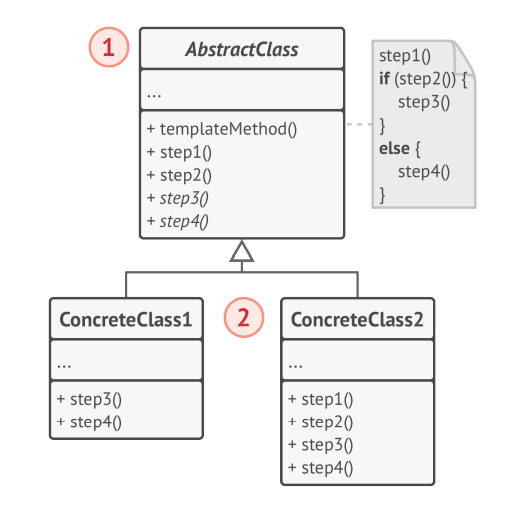
\includegraphics[scale=0.6]{image/behavioral/template.png}
\end{center}
\subsubsection{Ưu điểm và Nhược điểm}
Ta có rất nhiều ưu nhược điểm như sau:\\\\
Ưu điểm:
\begin{itemize}
    \item Các lớp con có thể thay đổi hoặc mở rộng các bước cụ thể của thuật toán mà không ảnh hưởng đến cấu trúc chung.
    \item  Mỗi bước của thuật toán được triển khai trong một phương thức riêng biệt, giúp tách rời và quản lý từng bước một.
    \item Cho phép người dùng override chỉ một số phần nhất định của thuật toán lớn, làm cho chúng ít bị ảnh hưởng hơn bởi những thay đổi xảy ra với các phần khác của thuật toán.
\end{itemize}
Nhược điểm:
\begin{itemize}
    \item Template method có càng nhiều bước để override càng khó bảo trì.
    \item Cần hiểu rõ khung (template) và cách các bước cụ thể được triển khai trong các lớp con.
\end{itemize}
\subsubsection{Code Example}
\begin{lstlisting}
#include <iostream>

// Abstract class defining the template method
class AbstractClass {
public:
    // Template method defining the algorithm
    void templateMethod() {
        step1();
        step2();
        step3();
    }

protected:
    virtual void step1() = 0;
    virtual void step2() = 0;
    virtual void step3() = 0;
};

// Concrete class implementing the template method
class ConcreteClass : public AbstractClass {
protected:
    void step1() override {
        std::cout << "ConcreteClass: Step 1" << std::endl;
    }

    void step2() override {
        std::cout << "ConcreteClass: Step 2" << std::endl;
    }

    void step3() override {
        std::cout << "ConcreteClass: Step 3" << std::endl;
    }
};

int main() {
    AbstractClass* abstractClass = new ConcreteClass();
    abstractClass->templateMethod();

    delete abstractClass;

    return 0;
}

\end{lstlisting}
Kết quả:
\begin{lstlisting}
ConcreteClass: Step 1
ConcreteClass: Step 2
ConcreteClass: Step 3
\end{lstlisting}
\subsubsection{Các Pattern liên quan}
\begin{itemize}
    \item Factory Method có thể đóng vai trò như một bước trong Template method là cơ sở chuyên môn hóa của Template Method.
\end{itemize}